\documentclass[preprint,12pt]{elsarticle}
\usepackage[T1]{fontenc}
\usepackage{lmodern}
\usepackage[a4paper,left=18mm,right=18mm,top=24mm,bottom=24mm]{geometry}
\usepackage{amsmath,amssymb,graphicx,booktabs,multirow,array,placeins}
\usepackage{algorithm,algpseudocode,xurl,hyperref}
\hypersetup{hidelinks,pdftitle={Sequential reference preservation for label-efficient set-valued prediction},pdfauthor={Xin Feng; Decong Yang}}
\biboptions{numbers,sort&compress}
\renewcommand{\bibfont}{\small}
\setlength{\bibsep}{3pt}
\renewcommand{\bibpreamble}{\interlinepenalty=10000}
\newcommand{\botrule}{\bottomrule}
\makeatletter
\newcommand{\raggedtablecolumns}{\let\savedarrayrestore\@arrayparboxrestore\def\@arrayparboxrestore{\savedarrayrestore\raggedright\arraybackslash}}
\makeatother
\renewcommand{\topfraction}{0.9}
\renewcommand{\bottomfraction}{0.8}
\renewcommand{\textfraction}{0.08}
\renewcommand{\floatpagefraction}{0.85}
\setcounter{totalnumber}{4}
\emergencystretch=2em
\raggedbottom
\journal{International Journal of Approximate Reasoning}
\newcommand{\markdataset}[1]{\expandafter\def\csname dataset@#1\endcsname{}}
\let\originalbibitem\bibitem
\RenewDocumentCommand{\bibitem}{o m}{%
  \IfNoValueTF{#1}{\originalbibitem{#2}}{\originalbibitem[#1]{#2}}%
  \ifcsname dataset@#2\endcsname [dataset]\space\fi}
\markdataset{har}
\markdataset{dsads}
\markdataset{mhealth}
\markdataset{wisdm}
\markdataset{pamap}
\markdataset{realdisp}
\markdataset{hhar}
\markdataset{jrcdata}

\begin{document}
\begin{frontmatter}
\title{Sequential reference preservation for label-efficient set-valued prediction}
\author[aff1]{Xin Feng\fnref{orf}}
\author[aff1]{Decong Yang\corref{cor1}\fnref{ory}}
\ead{20232501525@stu.xju.edu.cn}
\affiliation[aff1]{organization={Xinjiang University},addressline={Youhao Campus, 499 Xibei Road, Shayibake District},city={Urumqi},postcode={830091},state={Xinjiang},country={China}}
\cortext[cor1]{Corresponding author}
\fntext[orf]{ORCID: \url{https://orcid.org/0009-0008-3242-7961}}
\fntext[ory]{ORCID: \url{https://orcid.org/0009-0009-9295-5149}}
\begin{abstract}
Calibration can require more labels than are needed to reproduce a set-valued predictor's decisions. We introduce a sequential reference-preservation procedure that acquires labels until it can retain the prediction sets of a fully labeled reference pool within a prescribed size tolerance. Joint rank calibration (JRC) calibrates hypergeometric quantile bounds over the complete query schedule. A rank count tracks sampled items below the reference rank, and an inclusion indicator records whether the reference-ranked item has appeared. Propagating their joint state evaluates crossings of both quantile boundaries on the same query path. The endpoint sets then turn quantile uncertainty into an observable cardinality difference on an unlabeled monitoring batch. Querying stops when this difference meets the tolerance. Under uniform sampling without replacement, one confidence event guarantees reference-set containment for every input and bounds mean enlargement on the monitoring batch. Evaluation uses 354 classifier cases on seven wearable datasets and 45 additional cases on Heterogeneity Human Activity Recognition (HHAR). At confidence error 0.05 and tolerance 0.5, JRC saves 23.67\% of reference labels on the University of Southern California Human Activity Dataset (USC-HAD), compared with 17.91\% for Bonferroni hypergeometric bounds, 11.74\% for a uniform-prior confidence sequence and 15.33\% for its strongest reported prior variant. HHAR savings reach 34.03\%, against 25.13\% for the fixed Beta$(9,1)$ comparator. The procedure makes prediction-set precision an operational criterion for allocating calibration labels.
\end{abstract}
\begin{keyword}
Set-valued prediction \sep Reference preservation \sep Sequential calibration \sep Finite-population inference \sep Label acquisition \sep Conformal prediction
\end{keyword}
\end{frontmatter}
\section{Introduction}
A prediction set represents uncertainty through the outcomes it retains. Conformal methods provide statistical validity for such sets \cite{vovk,angelopoulos}, with links to broader uncertainty representations \cite{cella2022}. Constructing the calibration reference can nevertheless require substantial labeling. We study a concrete acquisition question: how many labels are needed to preserve the prediction sets that a fully labeled reference pool would produce, while allowing only a specified average enlargement? This target makes the precision of the returned sets part of the acquisition decision.

The reference-preservation objective distinguishes the present task from three related lines of work. Ilyas et al.\ \cite{ilyas} optimize a cost combining acquired labels and prediction-set size under an i.i.d. model; our objective is to reproduce a fixed finite reference within a set-size tolerance. Confidence sequences \cite{howard2021,howard2022,wor} provide intervals valid across sampling times; here, endpoint prediction sets turn an interval into a task-specific stopping rule. Active risk-controlling prediction sets \cite{active2024} guide label acquisition toward a prediction-risk constraint; we require retention of the reference sets and control their additional candidate labels. These distinct targets determine both the stopping criterion and the guarantee being evaluated.

We develop joint rank calibration (JRC) as a reference-preserving acquisition procedure. Its construction combines finite-population rank inference with exact calibration over a declared query schedule \cite{cochran,jin}. A fixed classifier and score function define the reference quantile. Sequential label queries narrow its interval, and candidate-label scores on an unlabeled monitoring batch translate the endpoints into nested prediction sets. The mean cardinality difference measures the prediction choices that remain unresolved by the queried labels. Acquisition stops when this observable difference reaches the user's tolerance and returns the upper-endpoint sets.

The rank-state representation connects the two quantile boundaries to the same query path. One state component counts queried items ranked below the reference quantile; the other records whether the reference-ranked item has appeared. The lower boundary depends on their sum, while the upper boundary depends on the count alone. Propagating this state evaluates the probability of crossing either boundary over the declared checkpoints. This yields a calibrated interval family that can be reused across pools with the same design. The method's contribution is the resulting acquisition procedure: schedule-specific calibration supplies the confidence event, and prediction-set width supplies the stopping decision.

The contributions are:
\begin{enumerate}
\item A reference-preservation acquisition objective that couples containment of the complete-reference prediction sets with a bound on their average enlargement.
\item A computable calibration-and-stopping procedure that turns partial reference labels and unlabeled monitoring scores into an adaptive query count, with a joint containment and size guarantee under uniform sampling without replacement.
\item An evaluation on seven wearable datasets with 354 frozen classifier cases and an additional HHAR study with 45 cases, quantifying label savings, reference quality and the effects of the stopping tolerance and boundary construction.
\end{enumerate}
The formulation connects a probability budget for reference loss to a cardinality budget for additional candidate labels. The latter has a direct interpretation in decision space and is invariant to strictly increasing score transformations. Wearable activity recognition provides an application in which user heterogeneity and imperfect probability calibration make set precision consequential \cite{guo,ovadia}. The experiments compare JRC with Bonferroni hypergeometric bounds and the stated anytime-valid confidence-sequence variants under a common reference-pool and query protocol.

\section{Related work}
\subsection{Set-valued prediction and uncertainty representation}
Prediction sets make the trade-off between error control and output precision explicit. Least-ambiguous set-valued classification studies small sets subject to error constraints \cite{sadinle}, while conformal methods connect set construction to calibration ranks \cite{vovk,angelopoulos,romano}. Cella and Martin relate conformal prediction to consonant plausibility measures and examine validity for different prediction tasks \cite{cella2022}. The object considered here is the enclosure of a fixed reference predictor as its calibration labels become available.

User and distribution heterogeneity affect the calibration properties of that reference. Hierarchical prediction and methods beyond exchangeability provide tools for such settings \cite{dunn,barber}. Our acquisition target conditions on the chosen finite pool and refines its quantile through randomized label queries. This separates uncertainty about the reference threshold from the ambiguity represented by the reference sets themselves.

\subsection{Sequential inference and label acquisition}

Ilyas et al. \cite{ilyas} study a stream of $n$ independent and identically distributed (i.i.d.) examples and the cost
\begin{equation}
 C(m)=m+(n-m)\,\mathbb E[|T_m(X)|]/K.
 \label{eq:relatedcost}
\end{equation}
Their procedure estimates normalized set size from candidate-label scores on unlabeled inputs and stops using a lower confidence bound on the cost increment. The regret analysis uses a monotone score-density-ratio assumption. The original-submission manuscript also describes a finite-sample stabilization for the experiments. These ideas motivate stopping decisions based on the observable size of prediction sets.

JRC targets containment of the prediction sets defined by a fixed reference pool. Its confidence statement is conditional on that pool and the uniform query order, with an additional size constraint on the monitoring batch. Table~\ref{tab:related} summarizes the statistical targets of the related approaches. The Ilyas comparison follows the original-submission version and distinguishes its theoretical stopping rule from the experimental stabilization.

Training-conditional validity has a longer history \cite{vovk2012}. Liang et al. study conformal inference with early stopping of neural-network training and reuse of hold-out data \cite{liangstop}. Xu et al. develop active, anytime-valid risk-controlling sets using a labeling policy and risk-predictor assistance \cite{active2024}. The August 2026 preprint by Skalse et al.\ \cite{skalse2026} studies a game with prediction and label-query actions on non-independent streams. Together, these studies address limited labeling resources through several population-risk and sequential-decision objectives.


\begin{table}[!htbp]
\centering\small\setlength{\tabcolsep}{4pt}
\raggedtablecolumns
\caption{Related statistical targets and acquisition decisions}\label{tab:related}
\begin{tabular}{p{24mm}p{38mm}p{42mm}p{44mm}}
\toprule
Procedure & Sampling target & Stopping or acquisition decision & Guarantee considered \\
\midrule
Ilyas et al.\ \cite{ilyas} & I.i.d. data-generating distribution & Cost-increment rule; empirical set size estimated from unlabeled inputs & Population coverage; asymptotic cost regret under a density-ratio condition \\
Howard and Ramdas\ \cite{howard2022} & Population quantiles from an i.i.d. stream & Any stopping time supported by the confidence sequence & Time-uniform confidence intervals for quantiles and distribution functions \\
Waudby-Smith and Ramdas\ \cite{wor} & Fixed population sampled without replacement & User-selected stopping applied to a confidence sequence & Time-uniform confidence sets for finite-population parameters \\
JRC & Corrected order statistic of a fixed finite reference pool & Endpoint set-size difference below a batch-specific tolerance & Reference-set containment for all inputs; average inflation control on the monitoring batch \\
\botrule
\end{tabular}
\begin{minipage}{\textwidth}\footnotesize All methods are compared under their stated sampling target and stopping contract.\end{minipage}
\end{table}


Finite-population sampling and hypergeometric inversion provide rank-inference tools \cite{cochran}. Confidence sequences \cite{howard2021,howard2022,wor} control sequential inspection, while exact group-sequential designs calibrate crossing probabilities on a chosen schedule \cite{jin}. The present procedure uses these principles to bound a fixed reference quantile and connects the bounds to an observable prediction-set stopping criterion.

\subsection{Wearable recognition as an evaluation setting}

Recent HAR frameworks improve representation learning and adaptation. STF-AL combines temporal, spatial and frequency representations with adversarial domain adaptation \cite{stfal}. CCT-HAR uses cross-modal sample mining and temporal alignment \cite{ccthar}, and TSDFSA studies attention-based feature selection for multiple sensors \cite{tsdfsa}. These methods motivate controlled evaluation of each component in a recognition pipeline. Our comparisons hold the trained classifier fixed to isolate the effect of calibration-label acquisition.

Uncertainty estimation is also important in HAR. Roy et al. study confidence-calibrated recognition \cite{roy}, and hyperdimensional computing combined with conformal prediction supports uncertainty-aware inference on microcontrollers \cite{hduq}. MiniRocket \cite{minirocket} and InceptionTime \cite{inception} provide established model families with contrasting representations. We use them to examine how acquisition behavior changes with the underlying score distribution.

\section{Finite-pool reference emulation}
\label{sec:method}

Figure~\ref{fig:1} shows the frozen-model and query workflow. The running extrema use the visited checkpoints, and both sums range over the monitoring batch. The checkpoint set in panel (b) denotes $\mathcal T$, whereas $T$ is the stopping query count. Algorithm~\ref{alg:jrc} specifies the acquisition procedure.

\begin{figure}[!htbp]\centering
\makebox[\textwidth][c]{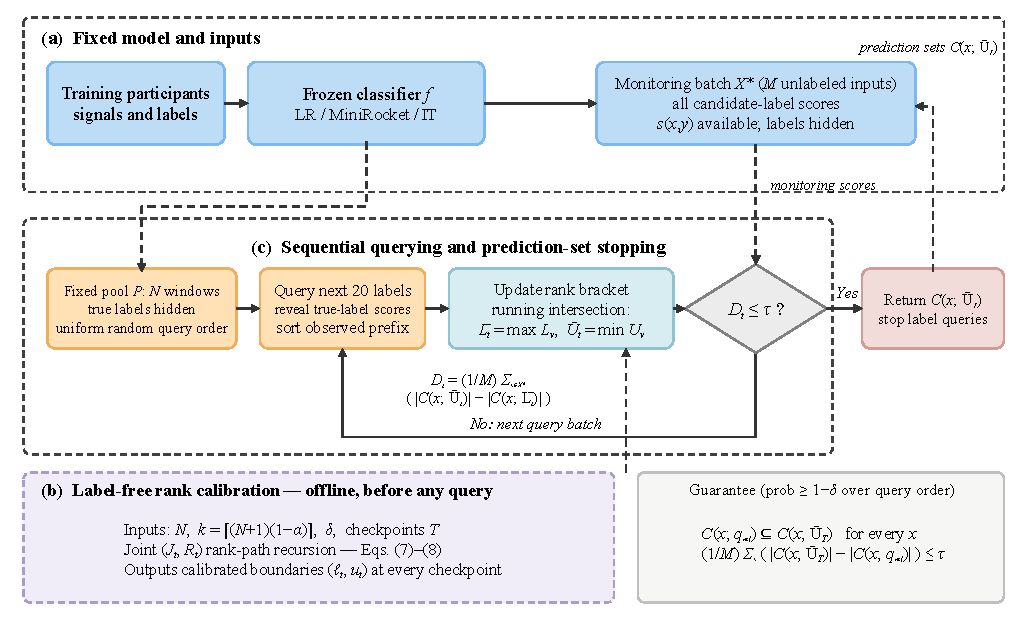
\includegraphics[width=174mm]{Fig1.pdf}}
\caption{JRC framework. (a) A frozen classifier provides candidate-label scores. (b) Joint rank calibration constructs checkpoint boundaries before querying. (c) Labels are queried uniformly without replacement to update the quantile bracket; querying stops when the endpoint sets meet the monitoring-batch size tolerance, and the upper-endpoint sets are returned}\label{fig:1}
\end{figure}

\subsection{Target, information and cost}
Let a trained classifier be fixed before calibration acquisition. For a nonconformity score $s(x,y)$, its thresholded prediction set is
\begin{equation}
 C(x;q)=\{y\in\mathcal Y:s(x,y)\le q\}.
 \label{eq:sets}
\end{equation}
The label set $\mathcal Y$ is finite, with $K$ classes. We fix a reference pool $\mathcal P=\{x_i\}_{i=1}^N$ before requesting its labels. The unknown true-label scores $S_i=s(x_i,y_i)$ are regarded as fixed values. Define
\begin{equation}
 k=\lceil(N+1)(1-\alpha)\rceil,\qquad
 q_{\rm ref}=S_{(k)},
 \label{eq:reference}
\end{equation}
with $q_{\rm ref}=+\infty$ if $k>N$. The predictor $C(x;q_{\rm ref})$ is the complete reference. Sequential acquisition aims to preserve these sets while using a subset of the pool labels. Population coverage is determined by the reference and its calibration assumptions; the probability statement below controls uncertainty arising from label acquisition.

We condition on all pool values, the trained classifier and a batch $\mathcal X_\star$ of $M$ unlabeled monitoring inputs. The probability statements concern a uniform permutation of the $N$ pool indices, selected independently of their unrevealed labels. This design accommodates dependencies among people, repeated windows and trials because inference conditions on the complete finite pool.

Candidate-label scores on $\mathcal X_\star$ are available before acquisition. They turn a quantile interval into an observable enclosure of the reference prediction sets. The stopping criterion controls the mean width of this enclosure on the monitoring batch.

The primary cost counts $T$ queried window labels. With $m$ reference participants and setup cost $c$ per participant, modeled effort is $T+cm$, compared with $N+cm$ for the complete reference. Both policies include all participant setup costs; signal collection, segmentation and pool construction precede acquisition.


\begin{algorithm}[t]
\caption{Joint rank calibration for a fixed reference pool}\label{alg:jrc}
\begin{algorithmic}[1]
\Require Frozen score function; fixed pool of $N$ windows; uniform query permutation; monitoring scores; $\alpha,\delta,\tau$; checkpoints $\mathcal T$
\State Set $k=\lceil(N+1)(1-\alpha)\rceil$ and calibrate rank boundaries $(\ell_t,u_t)$ by the joint recursion
\Statex \hspace{\algorithmicindent}\textit{Joint recursion: Section~\ref{sec:joint}, Eqs.~\eqref{eq:transition}--\eqref{eq:crossing}.}
\State Initialize observed scores $\mathcal S\gets\varnothing$, $L\gets-\infty$, $U\gets+\infty$
\For{each checkpoint $t\in\mathcal T$}
\State Query only the new labels needed to reach $t$ observations and add their true-label scores to $\mathcal S$
\State Obtain the current rank bracket $(L_t,U_t)$ from the ordered observed scores
\State Form $(L',U')\gets(\max\{L,L_t\},\min\{U,U_t\})$
\If{$L'>U'$}
\State Record an empty-intersection event and use $(L',U')\gets(L_t,U_t)$
\EndIf
\State Set $(L,U)\gets(L',U')$ and calculate $D_t$ from the monitoring scores using Eq.~\eqref{eq:width}
\If{$D_t\le\tau$}
\State \Return queried count $t$ and predictor $C(x;U)$
\EndIf
\EndFor
\end{algorithmic}
\end{algorithm}

\subsection{Finite-population rank brackets}
Choose checkpoints $\mathcal T\subseteq\{1,\ldots,N\}$ with $N\in\mathcal T$. If scores tie, order the complete population by the pair $(S_i,i)$, using the fixed pool index to break ties. The numerical inequalities below remain valid when these pairs are projected onto their score values.

Let $J_t$ count the queried items whose full-population ranks are strictly below $k$, and let $R_t$ indicate whether the item of rank $k$ has appeared. Then $J_t+R_t$ counts sampled items with rank at most $k$. Their separate marginal distributions are
\begin{equation}
 \begin{aligned}
 J_t&\sim\operatorname{Hypergeom}(N,k-1,t),\\
 J_t+R_t&\sim\operatorname{Hypergeom}(N,k,t).
 \end{aligned}
 \label{eq:hg}
\end{equation}
Write $Q_p(N,a,t)$ for the smallest integer whose hypergeometric cumulative probability is at least $p$. At a common tail parameter $\eta$, use sample-rank boundaries
\begin{equation}
 \ell_t=Q_\eta(N,k,t),\quad
 u_t=Q_{1-\eta}(N,k-1,t)+1.
 \label{eq:ranks}
\end{equation}
For the ordered observed scores $S^{[t]}_{(j)}$, set
\begin{equation}
 L_t=S_{(\ell_t)}^{[t]},\qquad U_t=S_{(u_t)}^{[t]}.
 \label{eq:bracket}
\end{equation}
Here $\ell_t$ is the lower sample-rank index defined in Eq.~\eqref{eq:ranks}. The conventions are $S^{[t]}_{(0)}=-\infty$ and $S^{[t]}_{(t+1)}=+\infty$. At the census, both bounds are the known $S_{(k)}$. When $k>N$, both are $+\infty$ and the reference already contains every label.

On a path satisfying $J_t+R_t\ge\ell_t$ and $J_t<u_t$, at least $\ell_t$ observations have full rank at most $k$, while fewer than $u_t$ observations have rank below $k$. Consequently, $L_t\le q_{\rm ref}\le U_t$. A standard simultaneous-coverage construction uses $\eta=\delta/[2(|\mathcal T|-1)]$ and a union bound over the non-census checkpoints. The resulting Bonferroni hypergeometric (HG) brackets form the first baseline.

\subsection{Joint calibration of the checkpoint boundaries}\label{sec:joint}
We calibrate the probability of crossing either rank boundary over the full checkpoint sequence. Conditional on state $(J_t,R_t)=(j,r)$, the next observation has rank below $k$, equal to $k$, or above $k$, with probabilities
\begin{equation}
 \frac{k-1-j}{N-t},\qquad
 \frac{1-r}{N-t},\qquad
 \frac{N-k-t+j+r}{N-t},
 \label{eq:transition}
\end{equation}
respectively. They lead to states $(j+1,r)$, $(j,1)$ and $(j,r)$. Impossible transitions have probability zero. Start with mass one at $(0,0)$; propagate these probabilities and absorb mass at any checkpoint for which
\begin{equation}
 j+r<\ell_t\quad\text{or}\quad j\ge u_t.
 \label{eq:crossing}
\end{equation}
The absorbed mass $A(\eta)$ is the exact probability of at least one rank-boundary crossing under the finite query design. There are at most $2k$ states at each time. Direct propagation costs $O(Nk)$ operations and $O(k)$ working memory for a specified boundary family. It is performed before label queries and reused across pools with the same $N$, $k$, confidence level and checkpoints.

Increasing $\eta$ tightens the rank bracket and increases the crossing probability $A(\eta)$. We use 24 bisection steps and retain a feasible value satisfying $A(\eta)\le\delta-10^{-10}$. This implements exact group-sequential calibration \cite{jin} for the specified reference rank. The resulting tables are reusable across pools with the same finite query design.

\subsection{Stopping in prediction-set space}
Intersect valid past brackets by setting $\overline L_t=\max_{v\le t}L_v$ and $\overline U_t=\min_{v\le t}U_v$, where $v\in\mathcal T$. On the simultaneous coverage event this intersection contains $q_{\rm ref}$. An empty intersection signals that event has failed; the implementation records it and falls back to the current bracket. At the census it returns the exact quantile regardless of previous events.

The stopping statistic is observable without monitoring labels:
\begin{equation}
 D_t=\frac1M\sum_{x\in\mathcal X_\star}
 \bigl[|C(x;\overline U_t)|-|C(x;\overline L_t)|\bigr].
 \label{eq:width}
\end{equation}
For tolerance $\tau\ge0$, querying stops at the first checkpoint with $D_t\le\tau$ and returns $C(x;\overline U_T)$. The census guarantees termination. The tolerance counts additional candidate labels per monitoring input, so its interpretation is preserved by strictly increasing transformations of the score.

\textbf{Proposition 1 (reference preservation).}
For a fixed classifier, finite reference pool, monitoring batch and declared checkpoints, suppose the joint recursion yields $A(\eta)\le\delta$. Under uniform sampling without replacement, with probability at least $1-\delta$, the returned predictor satisfies simultaneously
\begin{equation}
 C(x;q_{\rm ref})\subseteq C(x;\overline U_T),
 \label{eq:containment}
\end{equation}
for every input $x$, and
\begin{equation}
 \frac1M\sum_{x\in\mathcal X_\star}
 \bigl[|C(x;\overline U_T)|-|C(x;q_{\rm ref})|\bigr]
 \le\tau.
 \label{eq:inflation}
\end{equation}
No independence assumption on the fixed score values is required.

\textit{Proof.} The recursion enumerates the law of the uniformly sampled rank path. Except on an event of probability $A(\eta)$, neither inequality in Eq.~\eqref{eq:crossing} holds at any checkpoint. The rank argument above gives $L_t\le q_{\rm ref}\le U_t$ simultaneously. Running intersections therefore contain $q_{\rm ref}$ and are nonempty. Since the sets in Eq.~\eqref{eq:sets} are nested in $q$, the upper endpoint gives Eq.~\eqref{eq:containment} for every input. The reference set lies between the sets at the lower and upper endpoints, so its extra-label difference is bounded pointwise by the summand in Eq.~\eqref{eq:width}. At the data-dependent stopping time, the average is at most $\tau$. The confidence event covers every checkpoint and hence also this stopping time.\hfill$\square$

On the confidence event, empirical coverage is at least that of the reference on any fixed labeled test collection. The confidence level applies to one campaign under the declared query design.

Strictly increasing score transformations preserve the rank ordering and every thresholded set membership, so they leave the query count and returned sets unchanged. This invariance provides an implementation check.

\subsection{Implementation and comparison methods}
Sorted monitoring scores allow Eq.~\eqref{eq:width} to be computed using two binary searches. Each checkpoint sorts the observed label scores. This direct implementation is adequate for the pool sizes studied; dynamic order-statistic structures could reduce repeated sorting for larger pools. Precomputed boundary tables are separate from per-pool query execution.

The interval methods share the reference pool, query order, upper-endpoint output and set-inflation tolerance. Their rank bounds satisfy the stated confidence requirement over their respective query schedules. This common acquisition procedure provides the basis for comparing label cost.

The second quantile-interval baseline inverts the prior-posterior ratio confidence sequence (CS) of Waudby-Smith and Ramdas \cite{wor}. A uniform prior on the number of successes in the population induces the ordered-prefix mixture likelihood $B(j+1,t-j+1)$. For a hypothesized population count $a$, divide this mixture likelihood by
\begin{equation}
 \mathcal L_t(a,j)=
 \frac{(a)_j\,(N-a)_{t-j}}{(N)_t},
 \label{eq:likelihood}
\end{equation}
where $(a)_j$ denotes a falling factorial. Invert the resulting e-process separately at counts $k$ and $k-1$, allotting each error $\delta/2$. The minimum accepted count at $k$ gives the lower sample rank; one plus the maximum accepted count at $k-1$ gives the upper rank. We use the same running intersection, checkpoints and prediction-set stopping tolerance as JRC. JRC is calibrated on the declared finite schedule, whereas the CS comparator is valid at every sampling time; this difference is part of the reported comparison.

We additionally compare ordinary conformal quantiles from fixed 25\%, 50\% and 75\% prefixes, and an upper hypergeometric bound at a single fixed 50\% look. The former have no reference-containment guarantee. The latter protects the reference at that fixed look but does not adapt label expenditure to a prescribed set-size tolerance. Diagnostic ablations omit time correction, omit running intersection, return a midpoint at the proposed stopping time, or use sparse checkpoints. Their different guarantees are kept explicit.
The one-look HG comparator queries $\lceil N/2\rceil$ labels and returns the upper endpoint of the same two-sided hypergeometric interval, with error 0.025 in each tail. Thus, ``50\% look'' identifies the query fraction. This comparator uses a more conservative upper endpoint than a one-sided bound assigning error 0.05 to the upper tail.

\section{Experimental design}
\label{sec:experiments}
\subsection{Data and development history}
The main evaluation includes six development datasets: UCI HAR \cite{har}, DSADS \cite{dsads}, MHEALTH \cite{mhealth}, WISDM \cite{wisdm}, PAMAP2 \cite{pamap} and REALDISP \cite{realdisp}. They contain 122 eligible participant identifiers and 54,482 retained windows. These datasets were examined during acquisition-policy development. Earlier risk-based and randomized-allocation rules showed poor tolerance transfer on PAMAP2 and REALDISP, motivating the fixed-reference target. Their protocols and aggregate negative results are retained in Supplementary material 1.

USC-HAD \cite{uschad} provides the main confirmation benchmark. The method, confidence level, primary tolerance, query schedule, preprocessing and splits were locally locked on 12 September 2026 before model predictions were available. All 14 participants meet the requirement of at least 120 retained windows, yielding 5,353 windows and 12 classes. The main seven-dataset study therefore contains 136 dataset-specific participant identifiers and 59,835 windows.

The selected input is three acceleration axes resampled to 128 time points. UCI HAR uses the release's 2.56-second total-acceleration windows, retaining alternate windows in the released subject order. DSADS uses five-second torso-acceleration segments. MHEALTH uses five-second chest windows; WISDM uses five-second smartphone-acceleration windows from its 18-activity release. PAMAP2 uses protocol chest acceleration, and REALDISP uses ideal-placement BACK acceleration. The original REALDISP manual places BACK third in the log, unlike the fifth position listed in the repository webpage summary; we follow the original manual. The retained sample counts and preprocessing provenance are included in Table~\ref{tab:data} and the supplement. Table~\ref{tab:data} records the window durations and sensor placements.

For USC-HAD, each original MAT trial remains separate. We take nonoverlapping 500-sample windows at the documented 100 Hz, retain acceleration columns 1--3, reject nonfinite windows and incomplete tails, and use anti-aliased polyphase resampling to 128 points. The acquisition study starts from the supplied trial segmentation. The filename convention supplies activity IDs. An independent schema audit finds one conflict: Subject14/a3t2.mat is activity 3 by filename but activity 2 (walking-left) in its internal metadata. Main labels follow the locked filename rule. A separate sensitivity excludes that trial, refitting classifiers whenever it occurs in training. Another file lacks the optional numeric activity field but has a matching activity-name string; it is retained. No exact duplicate signal arrays are found among the 840 trials. The main analysis and the exclusion sensitivity are both reported.


\begin{table}[!htbp]
\centering\small\setlength{\tabcolsep}{3pt}
\caption{Public datasets and retained samples}\label{tab:data}
\begin{tabular}{lrrrlr}
\toprule
Dataset & People & Windows & Classes & Selected signal & Seconds \\
\midrule
UCI HAR & 30 & 5,155 & 6 & Waist total acceleration & 2.56 \\
DSADS & 8 & 9,120 & 19 & Torso acceleration & 5 \\
MHEALTH & 10 & 1,335 & 12 & Chest acceleration & 5 \\
WISDM & 51 & 32,653 & 18 & Phone acceleration & 5 \\
PAMAP2 & 8 & 3,775 & 12 & Chest acceleration & 5 \\
REALDISP & 15 & 2,444 & 33 & BACK acceleration & 5 \\
USC-HAD & 14 & 5,353 & 12 & Front right hip acceleration & 5 \\
\botrule
\end{tabular}
\begin{minipage}{\textwidth}\footnotesize The first six datasets are developmental; USC-HAD is the locked confirmation. Counts follow the fixed preprocessing before schema sensitivity.\end{minipage}
\end{table}

\subsection{Frozen classifiers and subject partitions}
Every acquisition method uses identical probability vectors within a classifier case. Logistic regression (LR) uses 35 standardized statistical features, regularization $C=1$ and a maximum of 2,000 iterations. MiniRocket (MR) uses 2,016 kernels followed by a standardized logistic-regression head. The InceptionTime-style model (IT) uses six modules, 32 filters per branch, kernel lengths 39, 19 and 9, residual connections every third module, global pooling and a classification head. It is trained for 40 epochs with Adam, learning rate $10^{-3}$ and batches of 128, without a test-selected checkpoint. The statistical features, normalization and model code are shared with the preceding frozen model study. Scikit-learn and SciPy support the classical pipeline \cite{sklearn,scipy}.

We reuse 249 cases from 83 outer partitions on the six development datasets. Each case has disjoint training, calibration and test participants. The acquisition procedure uses the frozen final-classifier predictions. USC-HAD has five fixed random seeds and seven test folds per seed: two test participants, eight training participants and four calibration participants in each fold. This gives 35 partitions and 105 new final-classifier fits. The 354 model cases reuse the 83 development and 35 confirmation partitions; repeated results are aggregated within participants.

The least ambiguous set-valued classifier (LAC) score \cite{sadinle} is $s(x,y)=1-\widehat p_y(x)$. The secondary score uses adaptive prediction sets (APS) \cite{romano} in a deterministic inclusive form: sort class probabilities in descending order, with stable class-index ties, and assign each class its cumulative probability. There is no randomization within the APS score and no forced top-label insertion. Empty and full sets remain in the calculations. The same scoring convention is used for the reference and every acquisition comparator, and $\alpha=0.1$ throughout.

\subsection{Reference pools and query experiments}
\noindent We construct each reference pool from $m$ calibration participants. The requested ceilings are $B\in\{120,240,480,960\}$, and the actual pool size is $N=\min(B,120m)$. Participant quotas differ by at most one; a random participant ordering allocates any remainder. Each quota is sampled uniformly without using its labels, after which the complete selected pool is independently permuted. When several ceilings produce the same pool size, the evaluation retains the declared configurations and reports their actual $N$.

The primary settings are confidence error $\delta=0.05$, mean set-inflation tolerance $\tau=0.5$, and checkpoints every 20 queried labels plus the census. The tolerance is measured in additional candidate labels per monitoring input. Secondary tolerances are 0.1, 0.25 and 1.0. Forty paired randomizations of pool selection and query order are used for each classifier case and ceiling. Every comparator shares the seeds, participants and windows. Complete labels define the evaluation reference; an oracle-based replay checks that acquisition decisions use only the labels already queried.

Test inputs supply the monitoring scores, with true labels hidden during acquisition. The stopping statistic and Window extra metric average over monitoring windows; reported coverage and set size give equal weight to participant summaries. Reference-label savings exclude training, segmentation and setup costs.

\subsection{Metrics, uncertainty and ablations}
Primary outcomes are queried-label savings $1-T/N$, reference-set containment failure and batch size inflation. A containment failure is the conservative scalar event $\overline U_T<q_{\rm ref}$; with ties or gaps in candidate scores, this can flag a threshold failure even when no observed test set loses a label. Bracket failure checks both endpoints. Size failure checks whether actual mean extra labels on the monitoring batch exceed $\tau$. Each query campaign is counted once, regardless of the number of held-out people.

For a test participant with empirical coverage $c_u$, positive shortfall is $(0.9-c_u)_+$. The positive part is calculated before averaging randomizations. Accuracy and macro-F1 describe the frozen point classifiers. Macro-F1 includes all activity classes, with zero contribution for undefined class scores. Subject summaries average paired randomizations and repeated partitions; paired 95\% bootstrap intervals resample these summaries within each dataset. The intervals therefore describe participant variation conditional on the fitted models and partitions. Sex and gender were not used for modeling or stratification, and performance within sex or gender groups was not assessed.

JRC, Bonferroni HG and the confidence sequence based on the prior-posterior ratio use identical tolerances and query checkpoints. Ablations remove the running intersection, use a sparse checkpoint grid, omit repeated-look correction or return the midpoint at the proposed stopping time. The uncorrected and midpoint variants serve as diagnostic controls. Fixed fractions and a one-look HG rule provide additional label-cost and set-size trade-offs. Exploratory checks vary $\delta$ and compare monitoring on even-indexed inputs with evaluation on odd-indexed inputs in the first MR case of each development dataset.

All runs use an Intel Core i9-12900HX CPU and an RTX 4070 Laptop GPU with 8 GB memory for neural training. We measure boundary-table construction separately from online acquisition calculations. Human annotation duration and device energy were outside the computational benchmark. Exhaustive small-population enumeration checks both rank engines and the coupled recursion; additional checks cover ties, census behavior, oracle access and strictly monotone score transformations.



\subsection{Additional HHAR confirmation}
After the main seven-dataset study, an additional Heterogeneity Human Activity Recognition (HHAR) confirmation \cite{hhar} was specified and publicly committed on 14 September 2026 before preprocessing outcomes or model fitting. The frozen method and classifier implementations were retained. All smartphone-accelerometer streams were processed separately by user and device. Five-second nonoverlapping windows were formed within activity-consistent runs, splitting at non-increasing timestamps or gaps above 0.5~s. Windows required at least 60 finite samples and 4.9~s of observed duration. Timestamp interpolation at 200~Hz followed by anti-aliased resampling produced 128 points. A label-blind random cap of 1,200 windows per user retained 10,800 windows from nine users and six classes. The fixed continuity filter retained very few Nexus4 windows. Device-specific retention counts are provided in Supplementary material~1.

Five declared seeds and three user-disjoint test folds used four training, two calibration and three test users per fold, yielding 45 additional LR, MR and IT cases. The primary analysis used LAC, $N=240$, $\delta=0.05$, $\tau=0.5$ and 40 paired query orders; $N=120$ and APS were secondary. Alongside Bonferroni HG, the fixed Beta$(9,1)$ confidence-sequence prior was a primary comparator, chosen from the preceding diagnostic before HHAR outcomes. User-level paired differences and 95\% bootstrap intervals follow the declared aggregation. This cohort is reported separately from the main USC-HAD confirmation.

\section{Results}
\subsection{Label savings against sequential quantile baselines}
Table~\ref{tab:primary} reports absolute reference utility and label savings for the three interval methods. Figure~\ref{fig:2} adds the secondary APS score. All three methods use the same nominal confidence error, tolerance, pool and query order. Their boundary constructions determine the observed acquisition costs. Figure~\ref{fig:2} averages the declared pool ceilings and participant summaries; paired uncertainty is reported in Section~\ref{sec:paired}.

\begin{table}[!htbp]
\centering\small\setlength{\tabcolsep}{3pt}
\caption{Primary LAC results at confidence error 0.05 and tolerance 0.5}\label{tab:primary}
\begin{tabular}{lrrrrrr}
\toprule
Dataset & Ref. cov. (\%) & Ref. size & Joint saved (\%) & HG saved (\%) & CS saved (\%) & Joint extra size \\
\midrule
UCI HAR & 90.45 & 1.035 & 71.62 & 64.93 & 58.97 & 0.235 \\
DSADS & 88.69 & 5.015 & 4.19 & 2.71 & 1.10 & 0.073 \\
MHEALTH & 89.07 & 1.459 & 45.17 & 38.25 & 30.92 & 0.206 \\
WISDM & 89.92 & 8.996 & 6.59 & 4.35 & 2.49 & 0.122 \\
PAMAP2 & 87.14 & 2.933 & 16.20 & 12.02 & 6.77 & 0.151 \\
REALDISP & 89.80 & 2.377 & 18.56 & 13.77 & 8.82 & 0.163 \\
USC-HAD & 90.36 & 2.590 & 23.67 & 17.91 & 11.74 & 0.179 \\
\botrule
\end{tabular}
\begin{minipage}{\textwidth}\footnotesize Saved (\%) is $100(1-T/N)$ relative to the full reference pool. Coverage, set size and extra size use equally weighted participant summaries; extra size is relative to the full reference. HG: Bonferroni hypergeometric; CS: prior-posterior rank confidence sequence.\end{minipage}
\end{table}

\begin{figure}[!htbp]\centering
\makebox[\textwidth][c]{\includegraphics[width=174mm]{Fig2.pdf}}
\caption{Reference-label savings at $\delta=0.05$ and $\tau=0.5$: (a) LAC; (b) APS. Bars show JRC, Bonferroni HG and the uniform-prior CS from left to right}\label{fig:2}
\end{figure}
On USC-HAD, the joint engine saves 23.67\% of reference labels, compared with 17.91\% for HG and 11.74\% for the uniform-prior CS. Its mean coverage is 91.80\%, against 90.36\% for the reference, and mean set size changes from 2.590 to 2.769. The coverage increase comes from the more inclusive calibration threshold; the point classifiers are unchanged.

Development-dataset savings range from 4.19\% on DSADS to 71.62\% on HAR; MHEALTH yields 45.17\% and WISDM 6.59\%. The width of the reference sets and the concentration of candidate scores near the reference quantile determine how quickly the endpoint sets meet the same tolerance.
\subsection{Reference preservation and absolute utility}
Table~\ref{tab:confirm} and Fig.~\ref{fig:3} compare fixed-fraction reductions with the quantile-interval baselines. Fixed fractions provide substantial label savings by construction, but their ordinary prefix quantiles need not contain the full-reference sets. A midpoint at a certified stopping time similarly discards the reason that upper-endpoint containment holds. The one-look HG rule returns the upper endpoint of a two-sided interval at the predetermined 50\% query fraction; it does not impose the adaptive set-inflation tolerance.

\begin{table}[!htbp]
\centering\small\setlength{\tabcolsep}{3pt}
\footnotesize
\caption{USC-HAD primary results and run-level failures}\label{tab:confirm}
\begin{tabular}{lrrrrrr}
\toprule
Policy & Saved (\%) & Coverage (\%) & Set size & Window extra & Threshold fail (\%) & Size fail (\%) \\
\midrule
Full reference & 0.00 & 90.36 & 2.590 & 0.0000 & 0.00 & 0.00 \\
Joint rank engine & 23.67 & 91.80 & 2.769 & 0.1824 & 2.04 & 0.72 \\
Bonferroni HG & 17.91 & 91.86 & 2.774 & 0.1870 & 0.45 & 0.21 \\
Uniform-prior CS & 11.74 & 91.76 & 2.761 & 0.1735 & 0.02 & 0.05 \\
Fixed 25\% & 75.00 & 90.46 & 2.713 & 0.1220 & 42.26 & 15.03 \\
Fixed 50\% & 50.00 & 90.41 & 2.632 & 0.0416 & 41.42 & 6.09 \\
Fixed 75\% & 25.00 & 90.36 & 2.601 & 0.0102 & 39.83 & 2.20 \\
One-look HG (50\% look) & 50.00 & 93.83 & 3.356 & 0.7737 & 1.73 & 46.64 \\
Midpoint output & 23.67 & 90.04 & 2.562 & -0.0282 & 46.40 & 0.14 \\
No time correction & 33.71 & 91.73 & 2.766 & 0.1784 & 6.29 & 3.02 \\
\botrule
\end{tabular}
\begin{minipage}{\textwidth}\footnotesize Saved (\%) is $100(1-T/N)$ relative to the full reference pool. Coverage and set size use participant weighting; Window extra is mean added set size over monitoring windows. Threshold fail: $\overline U_T<q_{\rm ref}$; Size fail: window inflation $>0.5$. Failure rates average query campaigns. One-look HG uses 2.5\% per tail and returns the upper endpoint.\end{minipage}
\end{table}

\begin{figure}[!htbp]\centering
\makebox[\textwidth][c]{\includegraphics[width=174mm]{Fig3.pdf}}
\caption{USC-HAD LAC failures: (a) threshold failure; (b) monitoring-batch inflation above 0.5 labels. Dashed line: $\delta=5\%$. Gray bars denote diagnostic rules; percentages denote query fractions. Mid: midpoint output; Uncorr.: uncorrected repeated looks}\label{fig:3}
\end{figure}
The proposed confirmation threshold-failure rate is 2.04\%, and its batch size-failure rate is 0.72\%. The confidence statement applies to one query campaign. A failure of the scalar threshold bracket may not remove any label on the finite observed input batch if no candidate score lies in the gap.

Reference quality and acquisition efficiency are connected. Coverage and set size in Tables~\ref{tab:primary} and \ref{tab:confirm} describe the predictor being preserved, while the savings and failure columns describe the additional acquisition procedure.
\subsection{Paired improvements and classifier dependence}\label{sec:paired}
Figure~\ref{fig:4} reports paired participant bootstrap intervals for additional savings against the quantile-interval baselines. These intervals condition on the fitted models and split collection. Table~\ref{tab:models} separates point-classification performance from acquisition outcomes for each confirmation backbone. Acquisition uses their frozen predictions.

\begin{figure}[!htbp]\centering
\makebox[\textwidth][c]{\includegraphics[width=174mm]{Fig4.pdf}}
\caption{Additional LAC label savings of JRC over (a) Bonferroni HG and (b) the uniform-prior CS. Points show paired participant means; bars show 95\% bootstrap intervals}\label{fig:4}
\end{figure}

\begin{table}[!htbp]
\centering\small\setlength{\tabcolsep}{3pt}
\caption{USC-HAD point-classifier and acquisition results}\label{tab:models}
\begin{tabular}{lrrrrr}
\toprule
Classifier & Accuracy (\%) & Macro-F1 (\%) & Labels saved (\%) & Set coverage (\%) & Set size \\
\midrule
LR & 60.17 & 56.14 & 32.85 & 92.76 & 2.769 \\
MR & 68.04 & 65.40 & 23.31 & 92.82 & 2.573 \\
IT & 65.14 & 60.32 & 14.85 & 89.83 & 2.967 \\
\botrule
\end{tabular}
\begin{minipage}{\textwidth}\footnotesize Each classifier has 35 outer partitions. IT is one InceptionTime-style network; macro-F1 includes all 12 classes.\end{minipage}
\end{table}
\subsection{Tolerance, query checkpoints and mechanism ablations}
Figure~\ref{fig:5} reports mean savings at all four tolerances declared before the USC-HAD results. Paired uncertainty at the primary tolerance is shown in Fig.~\ref{fig:4}. Relaxing the allowed average number of additional labels permits earlier stopping, as expected from Eq.~\eqref{eq:width}. The tolerance controls the permitted added ambiguity and the resulting cost-utility trade-off. The primary tolerance is 0.5.

\begin{figure}[!htbp]\centering
\makebox[\textwidth][c]{\includegraphics[width=174mm]{Fig5.pdf}}
\caption{Mean label savings of JRC versus the allowed extra set size: (a) LAC; (b) APS. Markers and line styles identify datasets}\label{fig:5}
\end{figure}
Table~\ref{tab:ablate} separates the mechanism choices. The first three rows retain their stated boundaries and checkpoints; midpoint and uncorrected variants are diagnostics. Removing running intersections reduces confirmation savings from 23.67\% to 21.10\%; sparse checkpoints reduce them to 16.84\%. Returning the midpoint retains the same label count but raises threshold failure to 46.40\%, illustrating why the protected upper endpoint is essential. Omitting repeated-look correction increases savings to 33.71\% and threshold failure to 6.29\%, above the declared 5\% error level.

\begin{table}[!htbp]
\centering\small\setlength{\tabcolsep}{3pt}
\caption{USC-HAD mechanism ablations}\label{tab:ablate}
\begin{tabular}{lrrrr}
\toprule
Rule & Saved (\%) & Extra size & Threshold fail (\%) & Size fail (\%) \\
\midrule
Joint rank engine & 23.67 & 0.179 & 2.04 & 0.72 \\
No intersection & 21.10 & 0.178 & 0.67 & 0.06 \\
Sparse checkpoints & 16.84 & 0.079 & 1.77 & 0.36 \\
Midpoint output & 23.67 & -0.028 & 46.40 & 0.14 \\
No time correction & 33.71 & 0.175 & 6.29 & 3.02 \\
\botrule
\end{tabular}
\begin{minipage}{\textwidth}\footnotesize Saved (\%) is $100(1-T/N)$ relative to the full reference pool. Extra size uses participant weighting and is relative to the reference. The first three rows retain their stated guarantees; midpoint and uncorrected rows are diagnostics.\end{minipage}
\end{table}
Figure~\ref{fig:6} traces the first declared USC-HAD MR query campaign at a 480-window pool. The trace uses the fixed first case. The census collapses all valid constructions to the same full-reference quantile, approximately 0.999436 in this example. The plotting floor is $10^{-16}$. Before that point, the mapping from rank uncertainty to set membership determines when each engine meets the tolerance.

\begin{figure}[!htbp]\centering
\makebox[\textwidth][c]{\includegraphics[width=174mm]{Fig6.pdf}}
\caption{USC-HAD MR query trace for LAC, $N=480$: (a) probability cutoff $1-\overline U_t$ on a logarithmic scale; (b) endpoint set-size difference, with stopping locations marked. Zero cutoffs and infinite upper bounds are plotted at $10^{-16}$. Horizontal line: $\tau=0.5$}\label{fig:6}
\end{figure}
Figure~\ref{fig:7} relates label savings to absolute reference set size and shows the corresponding reference and returned-set coverage pairs. Each dataset contributes LR, MR and IT points; their identities and values are provided in the model-summary table of Supplementary material~1.



\subsection{Sensitivity to stronger confidence-sequence priors}
The primary confidence-sequence baseline uses a uniform prior on the finite-population success count. After the main confirmation, we evaluated four fixed beta-binomial priors across all 354 existing classifier cases. A Beta$(a,b)$ mixture replaces the ordered-prefix mixture likelihood by $B(j+a,t-j+b)/B(a,b)$ while retaining the same likelihood-ratio construction and error allocation. Exact rank-path checks verify the error bound for each finite design used. The diagnostic reuses the main models and queries after confirmation; the locked JRC rule is unchanged.

Table~\ref{tab:priors} reports all four fixed prior choices. On USC-HAD, the strongest of these variants saves 15.33\% of labels, compared with 11.74\% for the uniform prior and 23.67\% for JRC. The variation demonstrates the role of boundary construction in acquisition efficiency under the declared settings. Reconstructing JRC and the uniform-prior results reproduces the archived dataset averages within $10^{-12}$.



\subsection{Schema exclusion and computation}
The exclusion sensitivity removes the USC-HAD trial with conflicting activity identifiers from every data role. The original classifier is reused only when that trial was absent from its training set; otherwise it is refitted. Joint-engine label savings change from 23.67\% to 22.70\%, coverage from 91.80\% to 92.30\%, and mean set size from 2.769 to 2.814. This check quantifies sensitivity to the trial-level label discrepancy.

Boundary tables depend only on the finite design and can be reused. Table~\ref{tab:runtime} separates table construction from execution with a cached table. Timings exclude JIT compilation, model inference and human labeling. Cached query execution includes sorting monitoring scores and observed prefixes. The timing benchmark uses a fixed score array and 1,000 unlabeled inputs with 12 candidate classes.


\begin{figure}[!htbp]\centering
\makebox[\textwidth][c]{\includegraphics[width=174mm]{Fig7.pdf}}
\caption{Reference utility for LAC: (a) label savings versus reference set size; (b) returned-set versus reference coverage. Each point is a dataset-classifier mean; color and shape identify datasets. The diagonal denotes equal coverage}\label{fig:7}
\end{figure}
\begin{table}[!htbp]\centering\small
\caption{Post-confirmation prior sensitivity: percentage of reference labels saved}\label{tab:priors}
\begin{tabular}{lrrrrr}
\toprule
Dataset & JRC & CS$(1,1)$ & CS$(0.5,0.5)$ & CS$(1.8,0.2)$ & CS$(9,1)$ \\
\midrule
UCI HAR & 71.62 & 58.97 & 60.85 & 66.89 & 64.84 \\
DSADS & 4.19 & 1.10 & 1.12 & 2.09 & 1.82 \\
MHEALTH & 45.17 & 30.92 & 32.06 & 36.58 & 36.51 \\
WISDM & 6.59 & 2.49 & 2.53 & 3.02 & 3.34 \\
PAMAP2 & 16.20 & 6.77 & 6.95 & 9.24 & 9.20 \\
REALDISP & 18.56 & 8.82 & 9.16 & 10.86 & 11.73 \\
USC-HAD & 23.67 & 11.74 & 12.01 & 14.22 & 15.33 \\
\botrule
\end{tabular}
\par\smallskip\begin{minipage}{\linewidth}\footnotesize LAC at $\delta=0.05$ and $\tau=0.5$. CS$(a,b)$ uses a Beta$(a,b)$ mixture; values use participant weighting. This diagnostic follows confirmation.\end{minipage}
\end{table}
\begin{table}[!htbp]\centering\small
\caption{Boundary construction and cached acquisition computation}\label{tab:runtime}
\begin{tabular}{lrrr}
\toprule
Pool size & Build table (ms) & Cached query loop (ms) & Exact crossing probability \\
\midrule
120 & 8.31 & 0.18 & 0.04843 \\
240 & 25.07 & 0.26 & 0.04606 \\
480 & 53.80 & 0.50 & 0.04991 \\
960 & 153.41 & 0.45 & 0.04981 \\
\botrule
\end{tabular}
\par\smallskip\begin{minipage}{\linewidth}\footnotesize Five repetitions on the stated CPU at $\delta=0.05$. Build time is per pool/checkpoint design; query time uses cached boundaries.\end{minipage}
\end{table}

\subsection{Additional HHAR confirmation}
Table~\ref{tab:hhar} reports HHAR label savings of 34.03\% for JRC, 28.58\% for HG and 25.13\% for the pre-specified Beta$(9,1)$ CS. Paired gains are 5.45 percentage points (95\% CI 5.09--5.85) against HG and 8.89 (8.52--9.23) against CS. These participant-bootstrap intervals condition on the fitted models and partitions.

Reference coverage and mean set size are 88.10\% and 1.807, versus 90.84\% and 1.997 for JRC. Table~\ref{tab:hhar} includes both failure rates; secondary pool-size, APS and classifier results are in Supplementary material~1.

\begin{table}[!htbp]\centering\small
\caption{Additional HHAR primary confirmation, $N=240$}\label{tab:hhar}
\begin{tabular}{lrrr}
\toprule
Policy & Saved (\%) & Threshold & Inflation \\
 & & fail (\%) & fail (\%) \\
\midrule
Reference & 0.00 & 0.00 & 0.00 \\
JRC & 34.03 & 1.33 & 0.28 \\
HG & 28.58 & 0.39 & 0.00 \\
CS$(9,1)$ & 25.13 & 0.28 & 0.00 \\
CS$(1,1)$ & 20.64 & 0.06 & 0.00 \\
\botrule
\end{tabular}
\par\smallskip\begin{minipage}{\linewidth}\footnotesize Saved (\%) is $100(1-T/N)$ relative to the full reference pool. CS$(a,b)$ denotes the Beta prior; failure rates count query campaigns.\end{minipage}
\end{table}
\FloatBarrier

\section{Discussion}
Reference preservation links sequential calibration to the precision of set-valued decisions. A rank bracket describes uncertainty about the reference threshold, while its endpoint sets describe the consequences of that uncertainty for prediction. Measuring their cardinality difference gives the stopping tolerance a direct interpretation: the average number of additional candidate labels presented to a decision maker.

The experiments characterize this trade-off across classifiers and datasets. Datasets with smaller reference sets generally admit larger savings in the evaluated settings. Candidate scores near the reference threshold determine how quantile uncertainty translates into extra labels. Boundary construction, prior choice and checkpoint frequency affect the acquisition path under the common reference-pool and query protocol.

The procedure operates with a fixed reference pool, uniform random queries and an available monitoring batch. These conditions make the rank law explicit and the stopping statistic observable. Further work can address grouped acquisition, changing monitoring batches and measured annotation effort. The current study reports queried-label counts and computation, with participant setup represented by the stated cost model.

\section{Conclusion}
Sequential reference preservation provides an acquisition target for set-valued prediction with costly calibration labels. The procedure combines finite-checkpoint rank calibration with a stopping criterion based on the precision of nested prediction sets. Its confidence event preserves the reference decisions and controls their average enlargement on the monitoring batch. The wearable evaluations show how query cost varies with the bound construction, classifier and reference-set quality. This connects a statistical error budget to a decision-level precision budget in a reproducible calibration workflow.

\section*{CRediT authorship contribution statement}
\textbf{Xin Feng:} Conceptualization, Methodology, Software, Data curation, Formal analysis, Investigation, Writing -- original draft. \textbf{Decong Yang:} Visualization, Writing -- review and editing.

\section*{Declaration of competing interest}
The authors declare that they have no known competing financial interests or personal relationships that could have appeared to influence the work reported in this paper.

\section*{Funding}
This research did not receive any specific grant from funding agencies in the public, commercial, or not-for-profit sectors.

\section*{Ethics and consent}
This study analyzes existing public benchmark data and involved no new participant recruitment or intervention.

\section*{Data availability}
The eight source datasets are available from the cited providers \cite{har,dsads,mhealth,wisdm,pamap,realdisp,uschad,hhar}. Frozen model predictions, query-campaign records, evaluation tables and protocols are publicly available in the versioned reproducibility archive \cite{jrcdata}. Supplementary material 1 contains the same scientific records together with verification results and reproduction instructions.

\section*{Code availability}
Code and reproduction instructions are available at \url{https://github.com/Cyrano666/jrc-reference-emulation}. The reported experiments use the archived implementation accompanying the frozen numerical records \cite{jrcdata}.

\section*{Supplementary material}
Supplementary material 1: reproduction code, frozen predictions, evaluation tables, protocols, verification records and editable figure sources.

\bibliographystyle{elsarticle-num}
\bibliography{references}
\end{document}
